\section{ساختار تصویربرداری \mri}\label{sec:mri-basics}

\subsection{تاریخچه}


تاریخچه تصویربرداری تشدید مفناطیسی
\LTRfootnote{Magnetic Resonance Imaging}(\mri)
تلاش تعداد زیادی از محققانی را شامل می‌شود که پدیده تشدید مغناطیسی هسته
\LTRfootnote{Nuclear Magnetic Resonance}(\lr{NMR})
را کشف کردند.
در سال ۱۹۵۰، حصول تصویر یک بعدی \mri توسط هرمن کار 
\LTRfootnote{Herman Carr}
 گزارش گردید. پاول لاتربر 
\LTRfootnote{Paul C. Lauterbur}
، شیمیدان آمریکایی با کار بر روی تحقیقات پیشین، موفق به ابداع روش‌هایی برای تولید تصاویر دو بعدی و سه بعدی \mri گردید. سرانجام وی در سال ۱۹۷۳ اولین تصویر گرفته شده بر اساس تشدید مغناطیس هسته‌ای (\lr{NMR}) خود را منتشر نمود. اولین تصویر مقطع نگاری از یک موش زنده در ژانویه ۱۹۷۴ منتشر گردید.


از سوی دیگر تحقیقات و پیشرفت‌های مهمی در زمینهٔ تصویر برداری بر اساس تشدید مغناطیسی هسته برای نخستین بار در دانشگاه ناتینگهام انگلستان 
\LTRfootnote{University of Nottingham}
صورت پذیرفت، جایی که پیتر منسفیلد فیزیکدان برجستهٔ آن مؤسسه با گسترش یک روش ریاضی موفق به کاهش زمان تصویربرداری و افزایش کیفت تصاویر نسبت به روش بکارگرفته شده توسط لاتربر گردید. در همان زمان در سال ۱۹۷۱ دانشمند آمریکایی ارمنی تبار ریموند دامادیان استاد دانشگاه ایالتی نیویورک در مقاله‌ای که در مجلهٔ Science منتشر گردید، اعلام نمود که امکان تشخیص تومور از بافت‌های عادی به کمک تصویر برداری 
\lr{NMR}
 میسر می‌باشد.

سرانجام جایزهٔ نوبل پزشکی سال ۲۰۰۳ به خاطر اختراع ام آر آی به پاول لاتربر از دانشگاه ایلینوی در اوربانا شامپاین و پیتر منزفیلد از انگلستان اعطا گردید. 
این جایزه به تنهایی می‌تواند اهمیت این نوع تصویربرداری را نشان دهد.

اما چه عواملی باعث شده‌اند تا این‌قدر \mri بااهمیت و ویژه باشند؟ تصویربرداری \mri روشی غیر تهاجمی و نسبتا امن است. 

سیستم‌های ام آر آی امروزه غالباً دارای قدرت میدان‌های ۰/۲، ۱، ۱/۵، و ۳ تسلا می‌باشند.
در ایالات متحده آمریکا بیمارستان‌ها و مراکز خدمات بهداشتی اجازه استفاده از سیستم‌های تا ۴ تسلا را نیز برای یک بیمار دارند. اما از چهار تسلا به بالا صرفاً جنبه و کاربردهای تحقیقاتی دارد.

امروزه بزرگ‌ترین تولیدکننده‌های سیستم‌های ام آر آی شرکت‌های زیمنس (آلمان)، جنرال الکتریک (آمریکا)، توشیبا (ژاپن)، و فیلیپس (هلند) می‌باشند.

\subsection{خطرات \mri}
برخلاف سایر دستگاه‌های تصویربرداری مثل اشعه ایکس و سی‌تی اسکن، ام آر آی از تشعشع یونیزه استفاده نمی‌کند. از این ابزار می‌توان برای تصویربرداری از جنین در دوران بارداری استفاده کرد بدون آن که اثری روی آن داشته باشد. اما باز هم این روش ممکن است خطراتی در پی داشته باشد و به همین دلیل جوامع پزشکی استفاده از \mri را در مراحل اولیه تشخیص بیماری توصیه نمی‌کنند. از آن‌جایی که در فرآیند ام آر آی از مغناطیس قوی استفاده می‌شود هر قطعه فلزی که در بدن وجود داشته باشد مثل ضربان ساز قلب، مفصل مصنوعی، دریچه مصنوعی قلب، حلزون مصنوعی گوش و یا هر نوع صفحه و پیچ و مهره فلزی در بدن ممکن است خطرساز باشد، چون میدان مغناطیسی می‌تواند باعث جابجایی و یا گرم شدن آن قطعه شود.

تعدادی از بیمارانی که از ضربان ساز قلب استفاده می‌کردند طی انجام ام آر آی از دنیا رفتند. بنابراین لازم است تکنولوژیست \mri سوالات لازم را قبل از انجام این فرآیند از بیمار بپرسد. البته بیشتر قطعات فلزی که امروز در ایمپلنت‌های بدن استفاده قرار می‌شوند تحت تأثیر میدان‌های مغناطیسی قرار نمی‌گیرند و به اصطلاح
\lr{MR-Safe}
 هستند. علاوه بر این، هنگام اسکن، دستگاه ام آر آی صداهای بلندی تولید می‌کند که ممکن است باعث ناراحتی فرد شود، بنابراین استفاده از حفاظ گوش در طول این فرآیند ضروری است.




\begin{figure}
	\centering
%	\copyrightbox[b]{
%	\begin{minipage}[c]{0.9\textwidth}
%	\centering
	\subfigure[تصویر پاول لاتربور]{
		\copyrightbox[b]{
		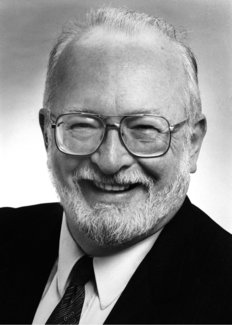
\includegraphics[height=0.35\linewidth]{figs/lauterbur-13686-content-portrait-mobile-tiny}
		}{\scriptsize{source:\url{https://is.gd/HgbMvo}}}
		\label{subfig:paullauterbur}
	}
	\hspace{0.1\linewidth}
	\subfigure[تصویر هرمن کار]{
		\copyrightbox[b]{
		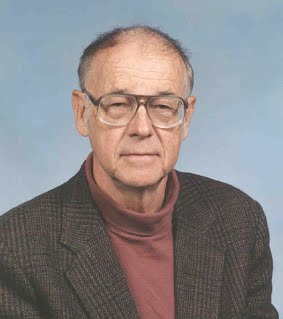
\includegraphics[height=0.35\linewidth]{figs/herman_carr}
		}{\scriptsize{source:\url{https://is.gd/teAHxS}}}
		\label{subfig:herman-carr}
	}
	\hspace{0.1\linewidth}
	\subfigure[تصویر Peter-Mansfield]{
		\copyrightbox[b]{
			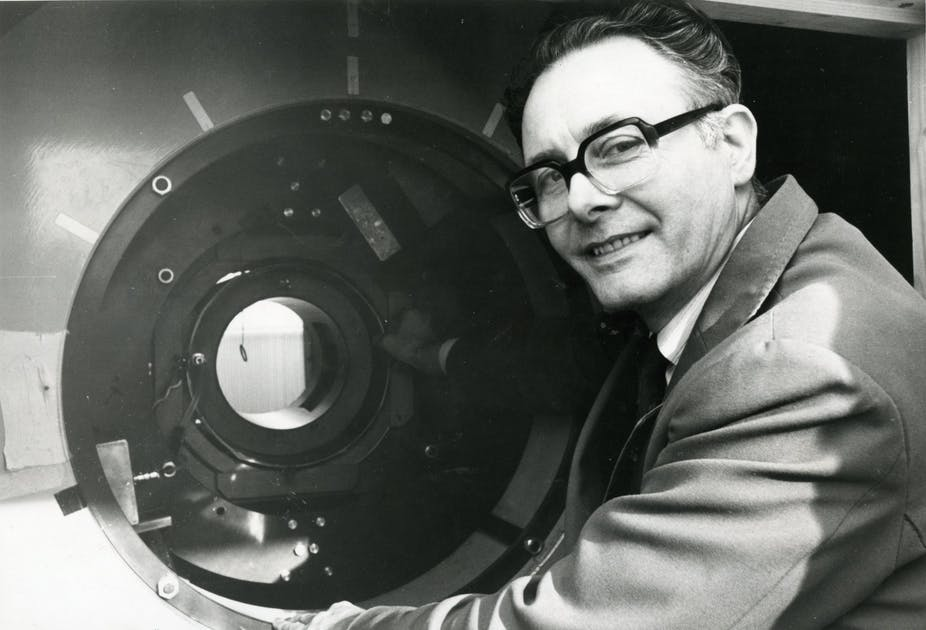
\includegraphics[height=0.3\linewidth]{figs/Peter-Mansfield}
		}{\scriptsize{source:\url{https://is.gd/W7AXIL}}}
		\label{subfig:Peter-Mansfield}
	}


%	\end{minipage}
%	}{\scriptsize\url{https://www.nobelprize.org/prizes/medicine/2003/lauterbur/biographical/}
%		\url{https://sites.google.com/a/pbsd.k12.pa.us/magnetic-resonance-imaging/herman-carr}
%		\url{https://theconversation.com/obituary-professor-sir-peter-mansfield-whose-invention-of-the-mri-scanner-revolutionised-medicine-72815}}
	\caption{تصویر سازندگان اصلی دستگاه تصویربرداری \mri}
	
	
\end{figure}



\begin{figure}
	\centering
	\copyrightbox[b]{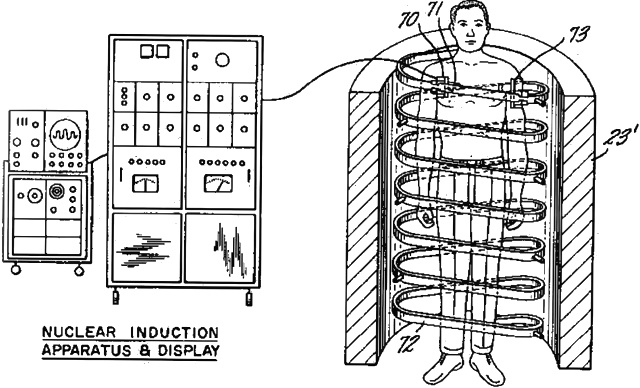
\includegraphics[width=0.7\linewidth]{figs/Damadian_invention}}
	{\url{https://en.wikipedia.org/wiki/File:Damadian_invention.jpg}}
	\caption{تصویری از آرشیو اداره ثبت اختراعات آمریکا که متعلق به ریموند دامادیان، دانشمند آمریکایی و یکی از مخترعین سیستم‌های نوین ام آر آی}
	\label{fig:Damadian_invention}
\end{figure}


\subsection{پدیده \nmr}
 

ساختار یک اتم، یک از اجزای اساسی در آزمایشات تشدید مغناطیسی است. اتم ها از سه ذره اصلی 
\LTRfootnote{Fundamental Particles}
تشکیلی شده اند:
\begin{enuminline}
	\item پروتون، که بار مثبت دارد
	\item نوترون، که بدون بار است
	\item الکترون، که بار الکتریکی منفی دارد
\end{enuminline}.


\begin{figure}
	\centering
%	\copyrightbox[b]{
		\subfigure[اسپین]{
		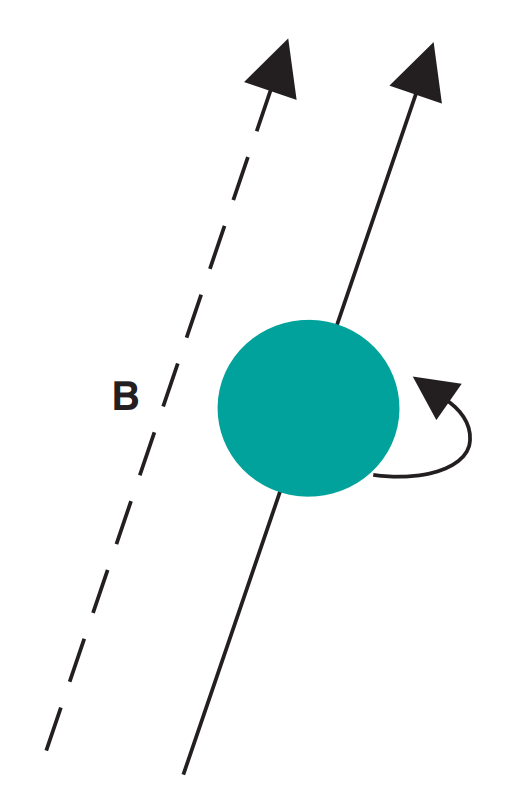
\includegraphics[height=0.3\linewidth]{figs/one-spin}
		\label{fig:one-spin}}
		\hspace{0.2\linewidth}
		\subfigure[مغناطیس]{
		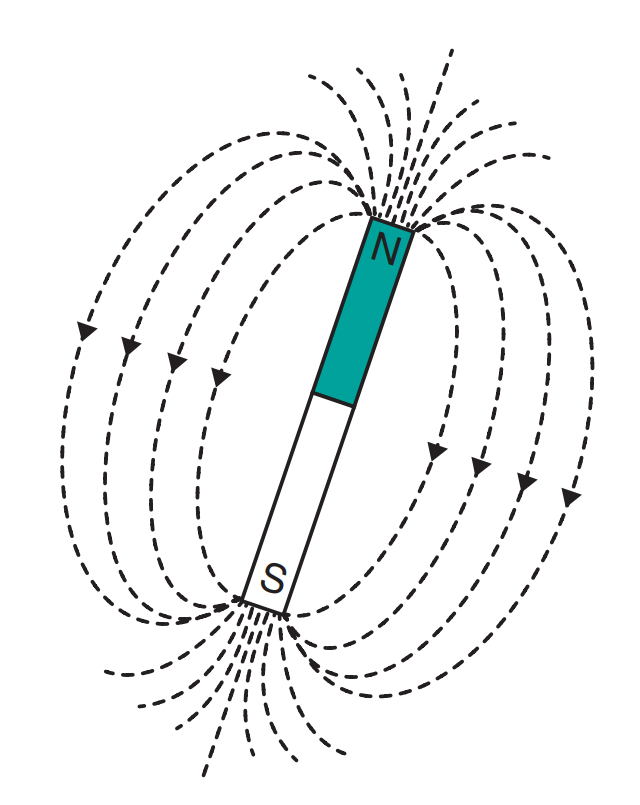
\includegraphics[height=0.3\linewidth]{figs/one-magnet}
		\label{fig:one-magnet}}
%	}{\cite{book:basic-principles-and-applications}}
	\caption{}
\end{figure}

\begin{figure}
	\centering
	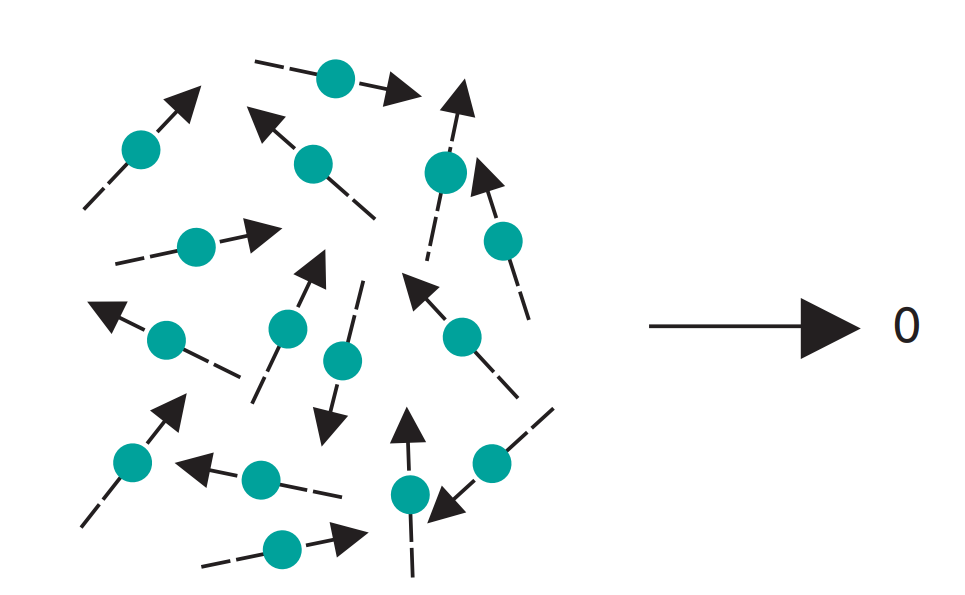
\includegraphics[width=0.7\linewidth]{figs/balance-spin}
	\caption{}
	\label{fig:balance-spin}
\end{figure}



\begin{figure}
	\centering
	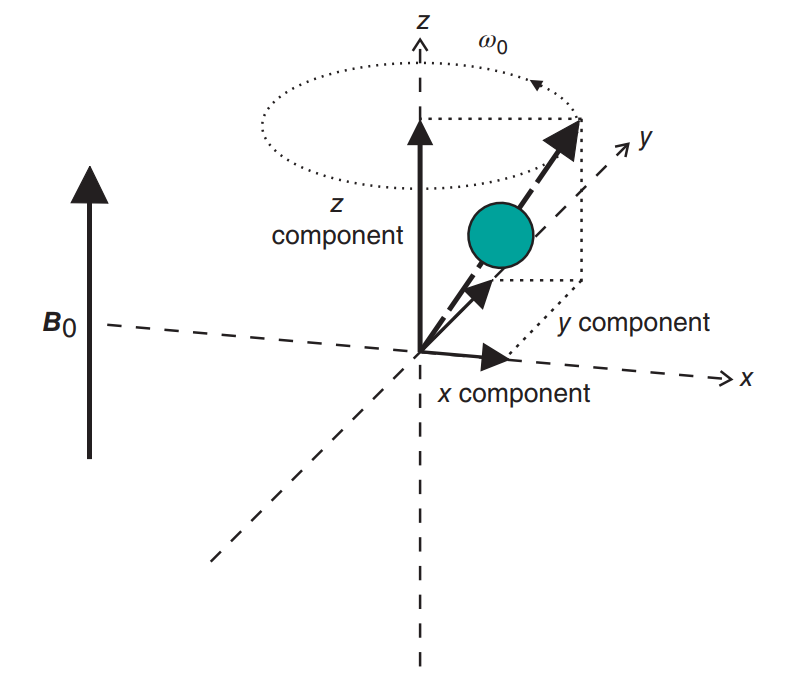
\includegraphics[width=0.6\linewidth]{figs/B-spin}
	\caption{}
	\label{fig:b-spin}
\end{figure}


\begin{figure}
	\centering
	\subfigure[]{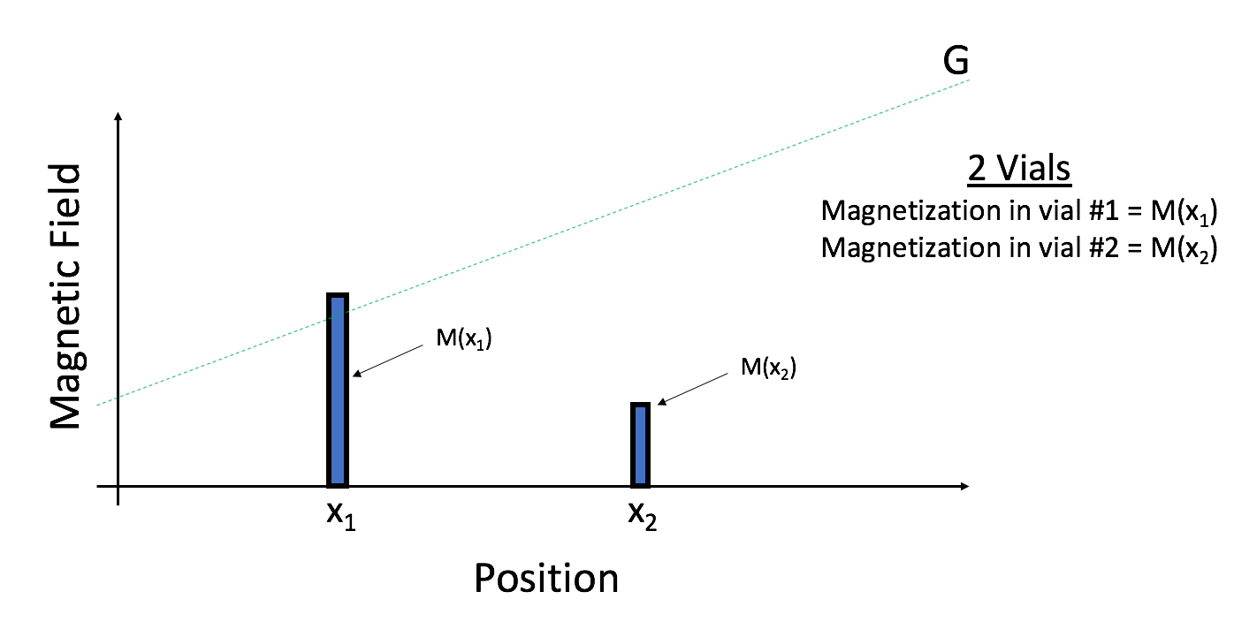
\includegraphics[height=0.23\linewidth]{figs/gr-1}\label{subfig:gr1}}
	\hspace{0.08\linewidth}
	\subfigure[]{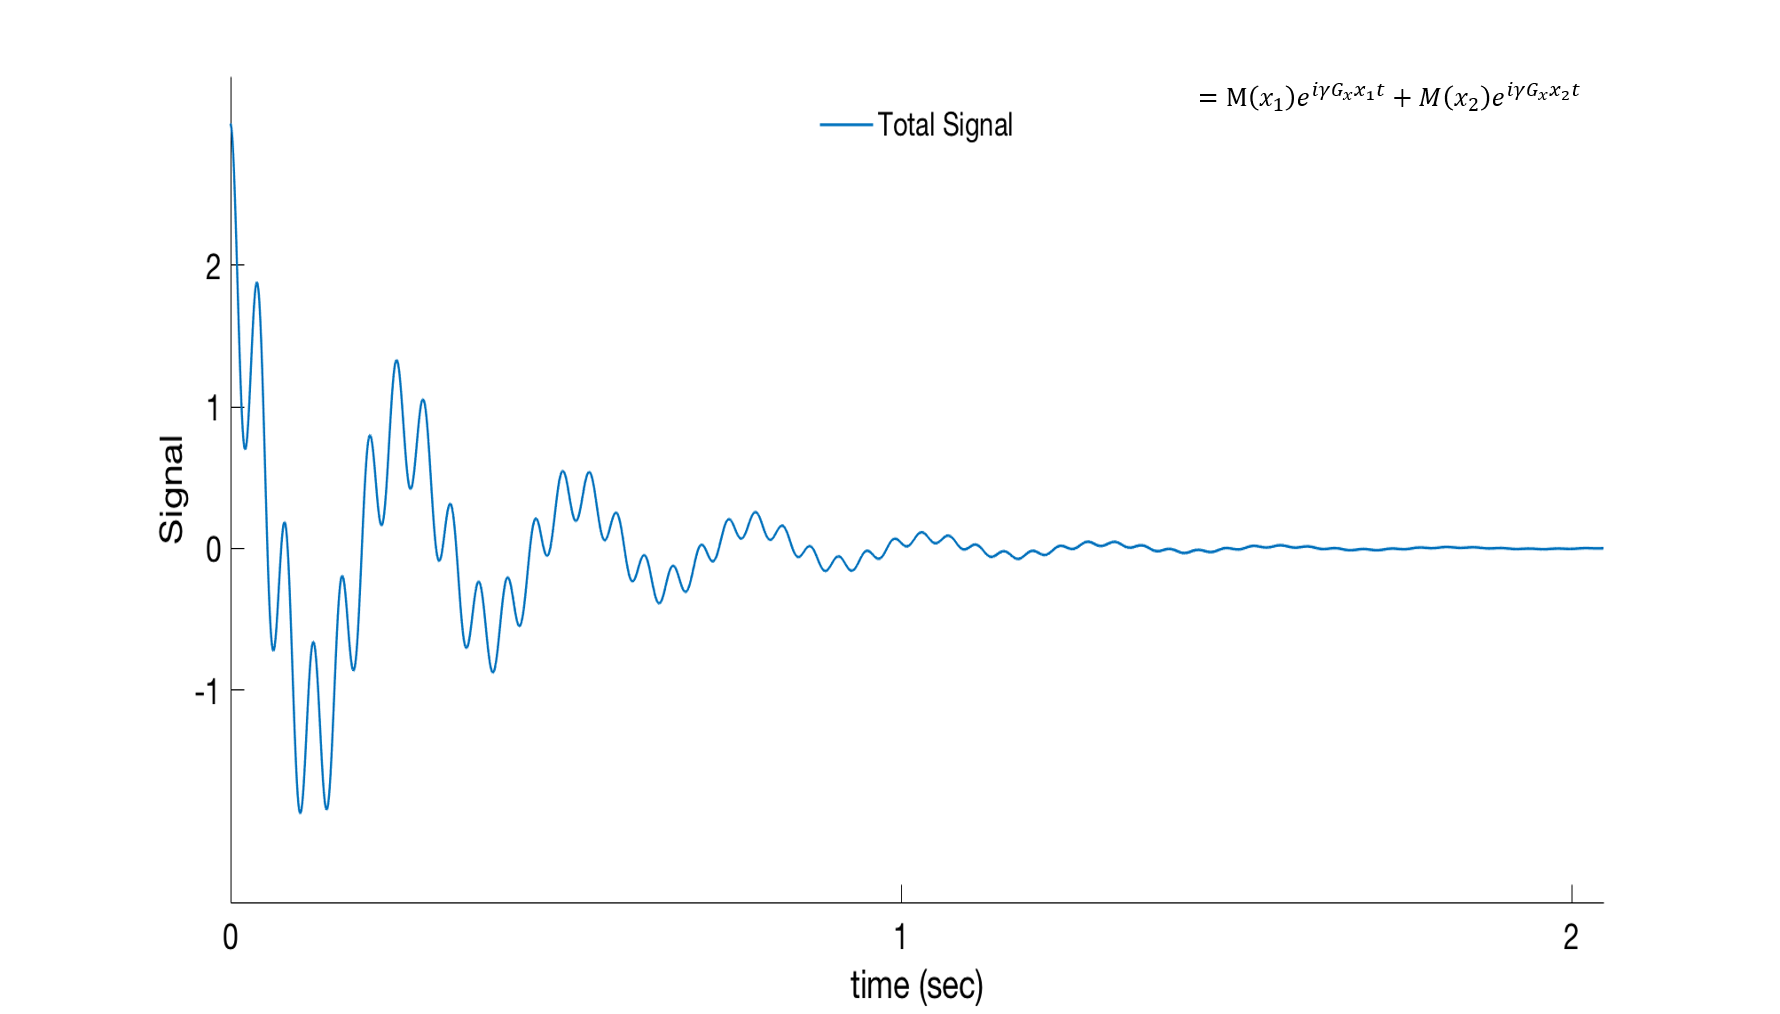
\includegraphics[height=0.23\linewidth]{figs/gr-3}\label{subfig:gr3}}
	\subfigure[]{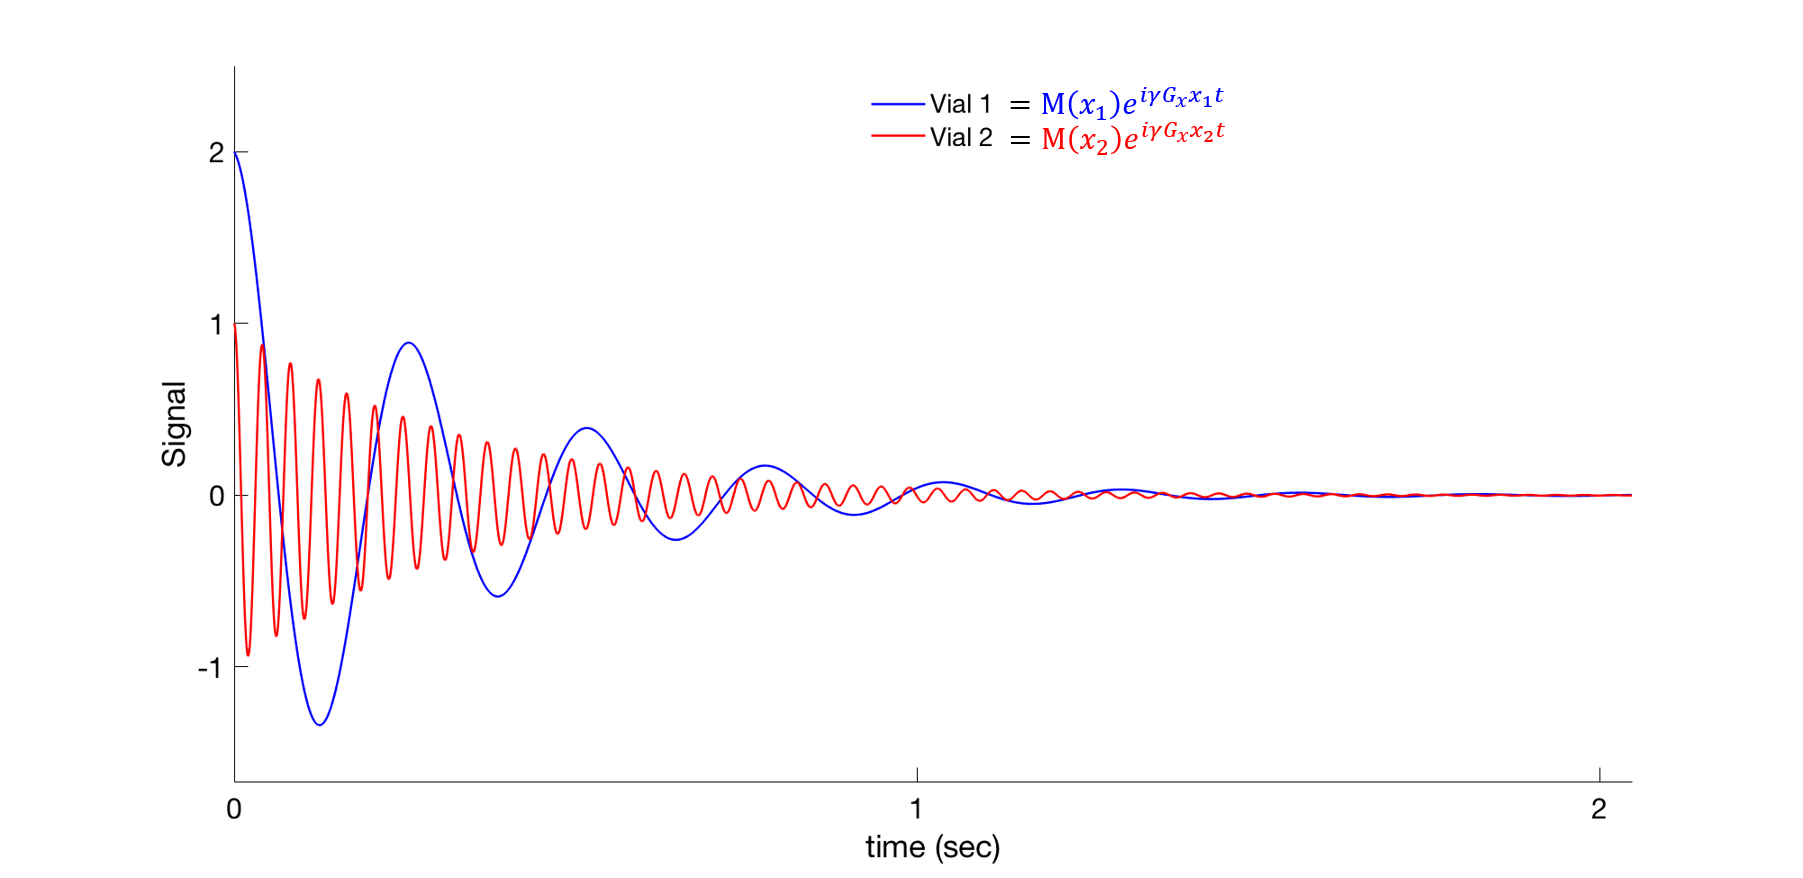
\includegraphics[height=0.23\linewidth]{figs/gr-2}\label{subfig:gr2}}
	\hspace{0.08\linewidth}
	\subfigure[]{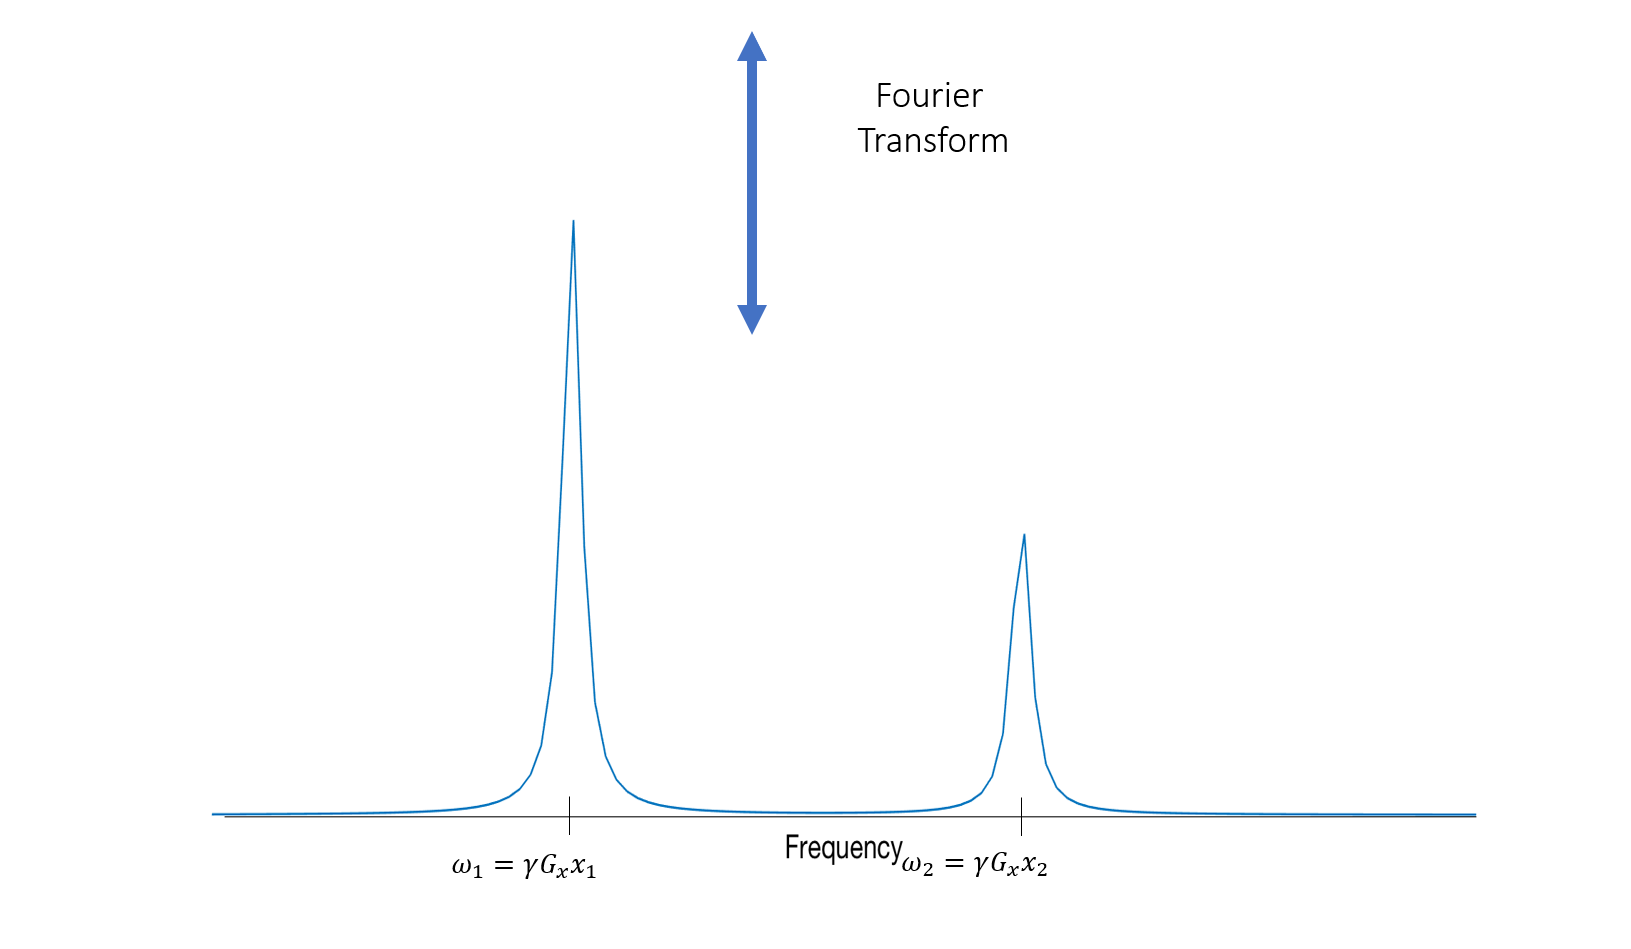
\includegraphics[height=0.25\linewidth]{figs/gr-4}\label{subfig:gr4}}
	\caption{}
	\label{fig:gr}
\end{figure}



\begin{figure}
	\centering
	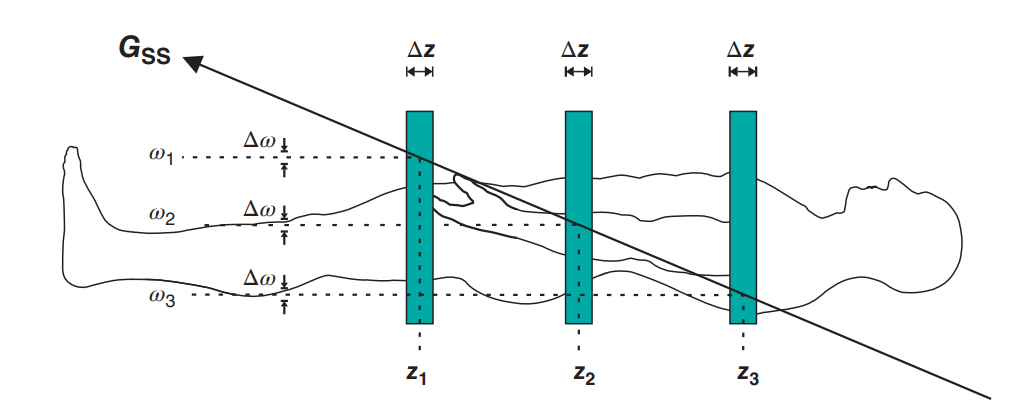
\includegraphics[width=0.7\linewidth]{figs/Slice-selection-process}
	\caption{}
	\label{fig:slice-selection-process}
\end{figure}

\begin{figure}
	\centering
	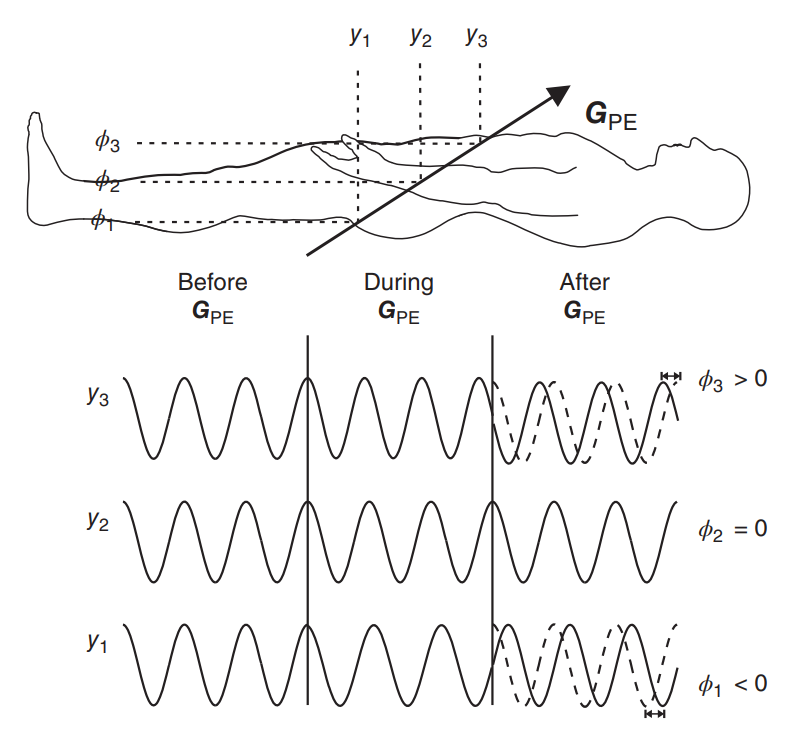
\includegraphics[width=0.7\linewidth]{figs/Concept-of-phase-encoding}
	\caption{}
	\label{fig:concept-of-phase-encoding}
\end{figure}













